\def\mytitle{MATRICES USING PYTHON}
\def\myauthor{V.GOKULKUMAR}
\def\contact{velicharlagokulkumar@gmail.com}
\def\mymodule{Future Wireless Communication (FWC)}
\documentclass[10pt, a4paper]{article}
\usepackage[a4paper,outer=1.5cm,inner=1.5cm,top=1.75cm,bottom=1.5cm]{geometry}
\twocolumn
\usepackage{graphicx}
\graphicspath{{./images/}}
\usepackage[colorlinks,linkcolor={black},citecolor={blue!80!black},urlcolor={blue!80!black}]{hyperref}
\usepackage[parfill]{parskip}
\usepackage{lmodern}
\usepackage{tikz}
	\usepackage{physics}
%\documentclass[tikz, border=2mm]{standalone}
\usepackage{karnaugh-map}
%\documentclass{article}
\usepackage{tabularx}
\usepackage{circuitikz}
\usetikzlibrary{calc}
\usepackage{amsmath}
\usepackage{amssymb}
\renewcommand*\familydefault{\sfdefault}
\usepackage{watermark}
\usepackage{lipsum}
\usepackage{xcolor}
\usepackage{listings}
\usepackage{float}
\usepackage{titlesec}
\providecommand{\mtx}[1]{\mathbf{#1}}
\titlespacing{\subsection}{1pt}{\parskip}{3pt}
\titlespacing{\subsubsection}{0pt}{\parskip}{-\parskip}
\titlespacing{\paragraph}{0pt}{\parskip}{\parskip}
\newcommand{\figuremacro}[5]{
    \begin{figure}[#1]
        \centering
        \includegraphics[width=#5\columnwidth]{#2}
        \caption[#3]{\textbf{#3}#4}
        \label{fig:#2}
    \end{figure}
}
\newcommand{\myvec}[1]{\ensuremath{\begin{pmatrix}#1\end{pmatrix}}}
\let\vec\mathbf
\lstset{
frame=single, 
breaklines=true,
columns=fullflexible
}
\thiswatermark{\centering \put(181,-119.0){
\includegraphics[scale=0.13]{iith_logo3}} }
\title{\mytitle}
\author{\myauthor\hspace{1em}\\\contact\\FWC22034\hspace{6.5em}IITH\hspace{0.5em}\mymodule\hspace{6em}September}
\date{}
\begin{document}
	\maketitle
	\tableofcontents
   \section{Problem}
  Let A be the centre of the circle $x^2 + y^2-2x-4y-20=0$. Suppose the tangents at the points  B(1,7) and D(4.-2) on the circle meet at the point C. Find the area of the quadrilateral ABCD.

   \section{Solution}
   The input parameters for this construction are 
\begin{center}
\begin{tabular}{|c|c|c|}
	\hline
	\textbf{Symbol}&\textbf{Value}&\textbf{Description}\\
	\hline
	r&5&Radius\\
	\hline
	A&\myvec{1\\2}& Centre\\
	\hline
    B&\myvec{1\\7}&Point B\\
	\hline
	D&\myvec{4\\-2}&Point D\\
	\hline
\end{tabular}
\end{center}
Circle equation : $x^2+y^2-2x-4y-20=0$   \\~\\
Equations of tangents at $\vec{B} , \vec{D}$ are given by
\begin{align}
x+7y-(x+1)-2(y+7)-20=0\\
%Equation of tangent at $\vec{B} \vec{D}$\\
4x-2y-(x+4)-2(y-2)-20=0
\end{align}
%$3x-4y=20$.............................(2)\\
The above equations result in the system 
\begin{align}
y=7\\
3x-4y=20
\end{align}
From (3),(4) let
\begin{align}
\vec{Z}=\myvec{0 & 1  \\
		3 & -4} \\   
\vec{X}=\myvec{7 \\ 20 }
\end{align}
Solve (5) and (6) \\
$\therefore$ Coordinates of C is  $\vec{C} = \myvec{16 \\ 7}$\\
Length of BC is  
	\begin{align}
			\vec{B}-\vec{C} &= \myvec{-15 \\ 0}\\
            \norm{\vec{B}-\vec{C}} &=\norm{\myvec{-15 \\ 0}}\\
			&=\sqrt{\myvec{-15 & 0}\myvec{-15 \\ 0}} \\
			&=15
\end{align}
Letting,
\begin{align}
\vec{v1}=\vec{A}-\vec{B}\\
\vec{v2}=\vec{A}-\vec{C}
\end{align}		
	Area of the $\Delta$ABC is given by 
	\begin{align}
&=\frac{1}{2}\norm{\vec{v1}\times\vec{v2}}
\end{align}
	Area of the of quadrilateral ABCD is given by 
	\begin{align}
&=2\times\frac{1}{2}\norm{\vec{v1}\times\vec{v2}}
\end{align}
$\therefore$The area of quadrilateral ABCD=75 sq.units\\~\\
\textbf{termux commands :}
\begin{lstlisting}
bash sh.sh
\end{lstlisting}
The below python code realizes the above construction:

\begin{lstlisting}
https://github.com/velicharlagokulkumar/FWC_module1/blob/main/matrices/circle/codes/matrix.py
\end{lstlisting}
 \section{Construction}
  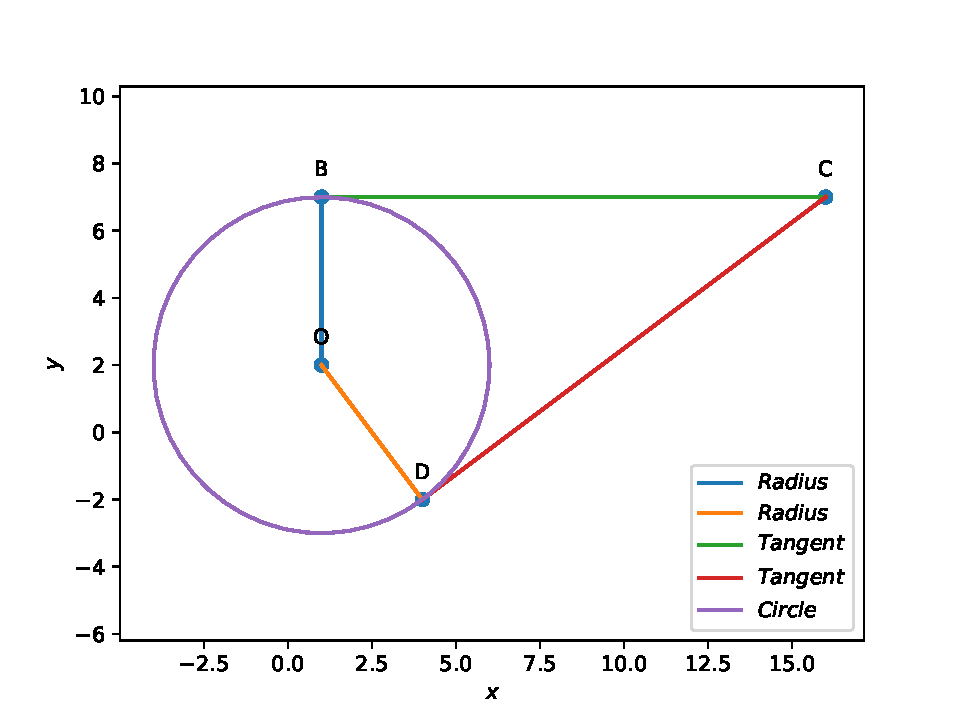
\includegraphics[scale=0.54]{matrix.pdf}
  	\begin{center}
  Figure of construction
  	\end{center}
%\bibliographystyle{ieeetr}
\end{document}